% Options for packages loaded elsewhere
\PassOptionsToPackage{unicode}{hyperref}
\PassOptionsToPackage{hyphens}{url}
%
\documentclass[
]{article}
\usepackage{amsmath,amssymb}
\usepackage{iftex}
\ifPDFTeX
  \usepackage[T1]{fontenc}
  \usepackage[utf8]{inputenc}
  \usepackage{textcomp} % provide euro and other symbols
\else % if luatex or xetex
  \usepackage{unicode-math} % this also loads fontspec
  \defaultfontfeatures{Scale=MatchLowercase}
  \defaultfontfeatures[\rmfamily]{Ligatures=TeX,Scale=1}
\fi
\usepackage{lmodern}
\ifPDFTeX\else
  % xetex/luatex font selection
\fi
% Use upquote if available, for straight quotes in verbatim environments
\IfFileExists{upquote.sty}{\usepackage{upquote}}{}
\IfFileExists{microtype.sty}{% use microtype if available
  \usepackage[]{microtype}
  \UseMicrotypeSet[protrusion]{basicmath} % disable protrusion for tt fonts
}{}
\makeatletter
\@ifundefined{KOMAClassName}{% if non-KOMA class
  \IfFileExists{parskip.sty}{%
    \usepackage{parskip}
  }{% else
    \setlength{\parindent}{0pt}
    \setlength{\parskip}{6pt plus 2pt minus 1pt}}
}{% if KOMA class
  \KOMAoptions{parskip=half}}
\makeatother
\usepackage{xcolor}
\usepackage{longtable,booktabs,array}
\usepackage{calc} % for calculating minipage widths
% Correct order of tables after \paragraph or \subparagraph
\usepackage{etoolbox}
\makeatletter
\patchcmd\longtable{\par}{\if@noskipsec\mbox{}\fi\par}{}{}
\makeatother
% Allow footnotes in longtable head/foot
\IfFileExists{footnotehyper.sty}{\usepackage{footnotehyper}}{\usepackage{footnote}}
\makesavenoteenv{longtable}
\usepackage{graphicx}
\makeatletter
\def\maxwidth{\ifdim\Gin@nat@width>\linewidth\linewidth\else\Gin@nat@width\fi}
\def\maxheight{\ifdim\Gin@nat@height>\textheight\textheight\else\Gin@nat@height\fi}
\makeatother
% Scale images if necessary, so that they will not overflow the page
% margins by default, and it is still possible to overwrite the defaults
% using explicit options in \includegraphics[width, height, ...]{}
\setkeys{Gin}{width=\maxwidth,height=\maxheight,keepaspectratio}
% Set default figure placement to htbp
\makeatletter
\def\fps@figure{htbp}
\makeatother
\setlength{\emergencystretch}{3em} % prevent overfull lines
\providecommand{\tightlist}{%
  \setlength{\itemsep}{0pt}\setlength{\parskip}{0pt}}
\setcounter{secnumdepth}{-\maxdimen} % remove section numbering
\ifLuaTeX
  \usepackage{selnolig}  % disable illegal ligatures
\fi
\IfFileExists{bookmark.sty}{\usepackage{bookmark}}{\usepackage{hyperref}}
\IfFileExists{xurl.sty}{\usepackage{xurl}}{} % add URL line breaks if available
\urlstyle{same}
\hypersetup{
  pdftitle={A Trace-Distance Error Bound for Stetcu--Baroni Filtering of a Matrix-Product Trial State},
  pdfauthor={Draft --- authors to be added},
  hidelinks,
  pdfcreator={LaTeX via pandoc}}

\title{A Trace-Distance Error Bound for Stetcu--Baroni Filtering of a
Matrix-Product Trial State}
\author{Draft --- authors to be added}
\date{7 October 2026}

\begin{document}
\maketitle

\hypertarget{abstract}{%
\subsection{Abstract}\label{abstract}}

A common hybrid recipe for ground-state preparation is to obtain a
matrix-product trial state and the low-lying energies classically
(DMRG), then repair the trial state's residual excited-state weight on a
quantum computer with the ancilla-based projection filter of Stetcu,
Baroni and Carlson. We give a short, fully explicit a-priori error bound
for this recipe. Writing \(D\) for the trace distance between the
prepared state and the exact ground state \(|E_0\rangle\), the bound is
a sum of two terms obtained from the triangle inequality: a
\emph{leakage} term, set by the trial-state ground-state weight
\(\gamma\) and a certified suppression factor \(\eta\) of the filter on
the excited spectrum, and a \emph{Trotter} term, set by a first-order
commutator constant \(\alpha\), the total evolution time \(T\) and the
number of Trotter steps \(n\). The bound needs only the trial state's
overlap, the spectral gap, the filter and the Hamiltonian's term
structure, and it converts to bounds on infidelity (\(D^2\)) and on the
energy error (\(W D^2\)). We test it on the open spin-½ \(J_1\)--\(J_2\)
chain for \(N=4\)--\(12\) with bond-dimension-2 trial states, by exact
simulation of the Trotterised filter. All 88 simulated points satisfy
every inequality. At the step count the bound prescribes for a target
\(D\le 0.1\), it overestimates the measured \(D\) by
\(2.7\)--\(4.9\times\): the leakage term is nearly tight
(\(1.3\)--\(2.5\times\)) while the Trotter term is conservative
(\(10\)--\(39\times\)), so the bound asks for \(11\)--\(60\times\) more
Trotter steps than are empirically needed. We also show where Pinsker's
inequality does and does not enter.

\hypertarget{introduction}{%
\subsection{1. Introduction}\label{introduction}}

DMRG gives, classically and cheaply, an accurate matrix-product state
(MPS) and estimates of the low-lying energies of a one-dimensional spin
chain. An MPS of modest bond dimension can be compiled into a shallow
circuit, but the resulting trial state \(|\psi\rangle\) has ground-state
weight \(\gamma=|\langle E_0|\psi\rangle|^2<1\). The projection
algorithm of Stetcu, Baroni and Carlson {[}1{]} (related to the rodeo
algorithm {[}2{]}) repairs this with one ancilla, controlled time
evolution under the Hamiltonian, and post-selection; the effect is to
multiply the trial state's energy components by a filter
\(F(E)=\prod_i\cos(Et_i+\phi_i)\).

The question this note answers is the practical one: \textbf{given a
trial state, the energies and a filter, how close is the prepared state
to \(|E_0\rangle\), and how many Trotter steps are enough?} We want an
answer that (i) is a theorem, (ii) uses only quantities a practitioner
has, (iii) fits in a few lines, and (iv) comes with empirical data
showing how conservative it is.

\textbf{Contributions.}

\begin{enumerate}
\def\labelenumi{\arabic{enumi}.}
\tightlist
\item
  A two-term bound \(D\le\sqrt{\bar\ell}+\epsilon_T/\sqrt{p_g}\) on the
  trace distance to the ground state (Theorem 1), proved from three
  elementary facts: trace distance of pure states is
  \(\sqrt{1-|\langle\cdot|\cdot\rangle|^2}\); it obeys the triangle
  inequality; and the leakage and Trotter errors can each be bounded
  separately. Corollaries give infidelity, energy error, and the number
  of Trotter steps.
\item
  An end-to-end workflow (Section 4) from trial state and energies to a
  certified step count.
\item
  An empirical study (Section 5): the bound is never violated, and we
  quantify which of its two terms is loose.
\item
  A short account of where Pinsker's inequality fits (Section 3.5),
  including why it cannot replace the triangle-inequality argument for a
  pure target.
\end{enumerate}

\textbf{What is not claimed.} The bound is first-order-Trotter only and
assumes the gap, \(\gamma\) and the ground energy are known (here: from
exact diagonalisation, \(N\le12\)). Hardware noise and gate synthesis
are not modelled. Section 6 lists the consequences. We report Trotter
steps, not gate counts; a companion cost study in this repository
(\texttt{evaluation/}) compares CX counts with direct MPS-circuit
preparation and finds no resource advantage for the filter on 1D chains
with \(N\le12\). This note does not revisit that conclusion.

\hypertarget{setting-and-notation}{%
\subsection{2. Setting and notation}\label{setting-and-notation}}

\textbf{Hamiltonian and energies.} \(H=\sum_{g=1}^{\Gamma}H_g\) is a sum
of \(\Gamma\) terms; for the open \(J_1\)--\(J_2\) chain each
\(H_g=J\,\mathbf S_i\!\cdot\!\mathbf S_j\) is one bond (\(j=i+1\) or
\(i+2\)). Let \(E_0<E_1\le\dots\le E_{\mathrm{top}}\) be the spectrum,
\(W=E_{\mathrm{top}}-E_0\) (any \(W\ge E_{\mathrm{top}}-E_0\) works),
and

\[H_s=\frac{H-E_0}{W},\qquad \operatorname{spec}(H_s)\subset\{0\}\cup[\Delta,1],\quad \Delta=\frac{E_1-E_0}{W}.\]

The ground state \(|g\rangle=|E_0\rangle\) is non-degenerate (even
\(N\), singlet).

\textbf{Trial state.} \(|\psi\rangle=\sum_kc_k|E_k\rangle\),
\(\gamma=|c_0|^2\).

\textbf{Filter.} One pulse acts on the system and an ancilla in
\(|0\rangle\):
\(\mathcal W(t,\phi)=\mathsf H_{\mathrm{a}}\,e^{-itH_s\otimes Z_{\mathrm{a}}}\,\mathrm{Rz}_{\mathrm{a}}(2\phi)\,\mathsf H_{\mathrm{a}}\),
and
\(\langle0_{\mathrm{a}}|\mathcal W|0_{\mathrm{a}}\rangle=\cos(H_st+\phi)\).
Keeping ancilla outcome \(0\) after each of \(m\) pulses
\((t_i,\phi_i)\) applies, up to normalisation,

\[F(E)=\prod_{i=1}^m\cos(Et_i+\phi_i),\qquad T=\sum_it_i,\qquad F(0)=\prod_i\cos\phi_i .\]

Define \(\eta=\sup_{E\in[\Delta,1]}|F(E)|/|F(0)|\) (smaller is better)
and \(p_g=\gamma F(0)^2\). The success probability is
\(P_{\mathrm{succ}}=\sum_k|c_k|^2F(E_k)^2\ge p_g\).

\textbf{Two states.} The \emph{ideal} filtered state is
\(|\varphi\rangle=F(H_s)|\psi\rangle/\|F(H_s)\psi\|\). The
\emph{implemented} state \(|\tilde\varphi\rangle\) replaces each
\(e^{-it_iH_s\otimes Z}\) by \(k_i\) first-order Lie--Trotter steps of
size \(dt=t_i/k_i\) over the terms \(H_g\) in a fixed order, with
\(n=\sum_ik_i\) and \(t_i=k_i\,dt\) (so \(T=n\,dt\)).

\textbf{Commutator constant.}
\(\alpha=\sum_{g}\big\|[H_g,\sum_{g'>g}H_{g'}]\big\|\) for \(H_s\) with
the terms in circuit order, taking the larger of the forward and
reversed order (so the bound does not depend on the product convention).
The ancilla does not change it, because
\([H_gZ,H_{g'}Z]=[H_g,H_{g'}]\otimes\mathbb 1\).

\begin{figure}
\centering
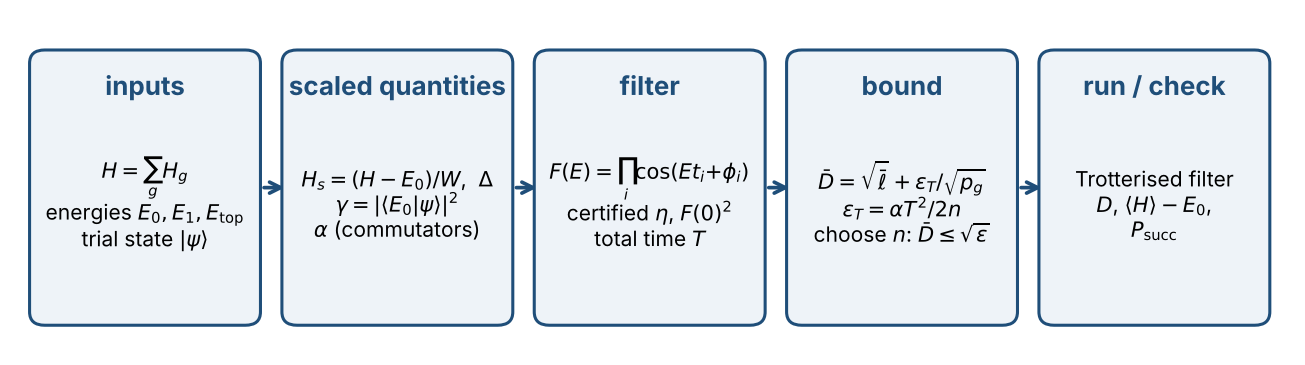
\includegraphics[width=1\textwidth,height=\textheight]{figs/fig_workflow.png}
\caption{Figure 1. Workflow: from trial state, energies and a filter to
a certified step count.}
\end{figure}

\hypertarget{the-bound}{%
\subsection{3. The bound}\label{the-bound}}

\hypertarget{trace-distance-the-triangle-inequality-and-fidelity}{%
\subsubsection{3.1 Trace distance, the triangle inequality, and
fidelity}\label{trace-distance-the-triangle-inequality-and-fidelity}}

For states \(\rho,\sigma\) let
\(D(\rho,\sigma)=\tfrac12\|\rho-\sigma\|_1=\tfrac12\operatorname{Tr}|\rho-\sigma|\).
Three facts are used.

\begin{itemize}
\tightlist
\item
  \textbf{(D1) Pure states.}
  \(D(|a\rangle\langle a|,|b\rangle\langle b|)=\sqrt{1-|\langle a|b\rangle|^2}=\sin\theta_{ab}\),
  where \(\theta_{ab}\) is the angle between the rays.
\item
  \textbf{(D2) Triangle inequality.}
  \(D(\rho,\tau)\le D(\rho,\sigma)+D(\sigma,\tau)\), since the trace
  norm is a norm.
\item
  \textbf{(D3) Fidelity (Fuchs--van de Graaf type).} For any state
  \(\rho\) and pure \(|g\rangle\),
  \(\;1-\langle g|\rho|g\rangle\le D(\rho,|g\rangle\langle g|)\le\sqrt{1-\langle g|\rho|g\rangle}\).
  For pure \(\rho\) the right-hand side is an equality, so infidelity
  \(=D^2\).
\end{itemize}

The lower bound in (D3) holds because
\(D\ge\operatorname{Tr}[|g\rangle\langle g|(\sigma-\rho)]\) with
\(\sigma=|g\rangle\langle g|\).

\hypertarget{leakage-how-well-would-an-exact-filter-do}{%
\subsubsection{3.2 Leakage: how well would an exact filter
do?}\label{leakage-how-well-would-an-exact-filter-do}}

\textbf{Lemma 1 (leakage).} If \(F(0)\ne0\), the ideal filtered state
satisfies
\[\ell:=1-|\langle g|\varphi\rangle|^2\;\le\;\bar\ell:=\frac{(1-\gamma)\,\eta^2}{\gamma+(1-\gamma)\,\eta^2},\qquad\text{so}\qquad D(\varphi,g)=\sqrt{\ell}\le\sqrt{\bar\ell}.\]

\emph{Proof.} The ground state sits at \(E=0\) in the scaled spectrum,
so \(|\langle g|\varphi\rangle|^2=\gamma F(0)^2/(\gamma F(0)^2+y)\) with
\(y=\sum_{k\ge1}|c_k|^2F(E_k)^2\). All \(E_k\), \(k\ge1\), lie in
\([\Delta,1]\), so \(F(E_k)^2\le\eta^2F(0)^2\) and
\(y\le(1-\gamma)\eta^2F(0)^2\). Since \(\ell=y/(\gamma F(0)^2+y)\) is
increasing in \(y\), substituting the bound for \(y\) gives the claim.
The equality \(D=\sqrt\ell\) is (D1). \(\square\)

\(\eta\) is \emph{certified} rather than sampled:
\(|F'|\le L:=\sum_i|t_i|\) and \(|F''|\le L^2\), so on an interval of
half-width \(d\) about \(E_c\),
\(|F(E)|\le|F(E_c)|+|F'(E_c)|d+\tfrac12L^2d^2\); interval bisection with
this envelope gives a rigorous upper bound on \(\sup_{[\Delta,1]}|F|\)
(\texttt{floor.certify}).

\hypertarget{trotter-error-of-the-post-selected-state}{%
\subsubsection{3.3 Trotter error of the post-selected
state}\label{trotter-error-of-the-post-selected-state}}

\textbf{Lemma 2 (Trotter).} Let
\(A_i=\langle0_{\mathrm{a}}|\mathcal W(t_i,\phi_i)|0_{\mathrm{a}}\rangle\)
and \(\tilde A_i\) the same block with \(k_i\) Trotter steps, and set
\(a=A_m\cdots A_1\psi\), \(b=\tilde A_m\cdots\tilde A_1\psi\)
(un-normalised). Then
\[\|a-b\|\le\epsilon_T:=\sum_{i=1}^m\frac{\alpha\,t_i^2}{2k_i}=\frac{\alpha T^2}{2n}\quad(t_i=k_i\,dt),\qquad D(\tilde\varphi,\varphi)\le\min\Big\{1,\frac{\epsilon_T}{\sqrt{p_g}}\Big\}.\]

\emph{Proof.} (i) The first-order product-formula bound (Appendix A,
following Childs et al.~{[}3{]}) gives
\(\|\mathcal W_i-\widetilde{\mathcal W}_i\|\le\alpha t_i^2/(2k_i)\).
(ii) \(A_i,\tilde A_i\) are compressions of
\(\mathcal W_i,\widetilde{\mathcal W}_i\) to the ancilla-\(|0\rangle\)
block, so
\(\|A_i-\tilde A_i\|\le\|\mathcal W_i-\widetilde{\mathcal W}_i\|\), and
\(\|A_i\|,\|\tilde A_i\|\le1\). (iii) Telescoping,
\(a-b=\sum_i(A_m\cdots A_{i+1})(A_i-\tilde A_i)(\tilde A_{i-1}\cdots\tilde A_1\psi)\),
so \(\|a-b\|\le\sum_i\epsilon_i\). (iv) The rays of \(a\) and \(b\) are
\(\varphi\) and \(\tilde\varphi\). By (D1),
\(D=\sin\angle(a,b)=\operatorname{dist}(a,\operatorname{span}b)/\|a\|\le\|a-b\|/\|a\|\),
and \(\|a\|^2=P_{\mathrm{succ}}\ge p_g\). \(\square\)

\hypertarget{the-bound-1}{%
\subsubsection{3.4 The bound}\label{the-bound-1}}

\textbf{Theorem 1.} Under the assumptions of Section 2,
\[\boxed{\;D(\tilde\varphi,g)\;\le\;\bar D:=\min\Big\{1,\;\sqrt{\bar\ell}+\frac{\alpha T^2}{2n\sqrt{\gamma F(0)^2}}\Big\}\;}\]

\emph{Proof.} Triangle inequality (D2):
\(D(\tilde\varphi,g)\le D(\tilde\varphi,\varphi)+D(\varphi,g)\). Bound
the first term by Lemma 2 and the second by Lemma 1. \(\square\)

\textbf{Corollary 1 (infidelity).}
\(1-|\langle g|\tilde\varphi\rangle|^2=D^2\le\bar D^2\).

\textbf{Corollary 2 (energy).}
\(\langle\tilde\varphi|H|\tilde\varphi\rangle-E_0\le W\,D^2\le W\bar D^2\).
\emph{Proof.} With \(\tilde c_k\) the components of \(\tilde\varphi\),
\(\sum_{k\ge1}|\tilde c_k|^2(E_k-E_0)\le W\sum_{k\ge1}|\tilde c_k|^2=W(1-|\tilde c_0|^2)=WD^2\).
\(\square\)

\textbf{Corollary 3 (step count).} For a target \(D\le\sqrt\varepsilon\)
and a certified \(\bar\ell<\varepsilon\), it suffices that
\[n\;\ge\;\frac{\alpha T^2}{2\sqrt{\gamma F(0)^2}\,\big(\sqrt\varepsilon-\sqrt{\bar\ell}\big)},\qquad\text{e.g. }\ n\ge\frac{\alpha T^2}{\sqrt{\gamma F(0)^2\,\varepsilon}}\ \text{ if }\bar\ell\le\varepsilon/4 .\]
Since \(T=x\pi/\Delta\) with \(x=O(1)\) chosen by the filter design,
\(n\propto\alpha/(\Delta^2\sqrt{\gamma F(0)^2\varepsilon})\).

The design problem is then: choose \((t_i,\phi_i)\) to maximise
\(F(0)^2\) (hence \(p_g\) and \(P_{\mathrm{succ}}\)) subject to
certified \(\eta\le\eta_*\), where
\(\eta_*^2=\gamma\varepsilon_\ell/((1-\varepsilon_\ell)(1-\gamma))\)
makes \(\bar\ell=\varepsilon_\ell\). We use the solver \texttt{floor.py}
for this.

\hypertarget{remarks-noise-tightness-and-pinsker}{%
\subsubsection{3.5 Remarks: noise, tightness, and
Pinsker}\label{remarks-noise-tightness-and-pinsker}}

\textbf{Mixed states and noise.} If the device prepares a mixed state
\(\tilde\rho\) (e.g.~with noise), (D2) still applies:
\(D(\tilde\rho,g)\le D(\tilde\rho,\tilde\varphi)+\bar D\). The
infidelity bound then degrades from \(D^2\) to \(D\) via (D3).

\textbf{Sharpening.} With angles instead of sines,
\(D\le\sin\!\big(\arcsin\sqrt{\bar\ell}+\arcsin(\epsilon_T/\sqrt{p_g})\big)\)
whenever the sum of angles is at most \(\pi/2\). It is slightly tighter
and no harder to compute; we keep the additive form because it is the
one that reads off as ``leakage plus Trotter''.

\textbf{Pinsker.} For the \emph{target} \(|g\rangle\langle g|\),
Pinsker's inequality \(D\le\sqrt{S(\rho\|\sigma)/2}\) is vacuous in the
useful direction: \(S(\rho\|\,|g\rangle\langle g|)=+\infty\) unless
\(\rho=|g\rangle\langle g|\), because \(\rho\) has support outside a
pure state. This is why the argument above goes through fidelity and the
triangle inequality rather than relative entropy. Pinsker does enter if
one looks at the \emph{energy-resolved distributions} \(p_k=|c_k|^2\)
(trial) and \(q_k=p_kF(E_k)^2/P_{\mathrm{succ}}\) (ideally filtered),
for which

\[\mathrm{KL}(q\|p)=\sum_kq_k\ln\frac{F(E_k)^2}{P_{\mathrm{succ}}}\le\ln\frac1{P_{\mathrm{succ}}}\quad(|F|\le1),\qquad \mathrm{TV}(p,q)\le\sqrt{\tfrac12\mathrm{KL}(q\|p)},\]

while \(\mathrm{TV}(p,q)\ge q_0-p_0=1-\ell-\gamma\). Together,
\[P_{\mathrm{succ}}\;\le\;\exp\!\big(-2(1-\ell-\gamma)^2\big):\]
post-selection cannot be free if the filter is to move weight from
\(\gamma\) to \(1-\ell\). This is a necessary condition on the cost, not
an error bound, and (Section 5.7) it is weak for the cases studied. We
include it to mark where relative-entropy tools apply and to be explicit
that they do not drive the main result.

\hypertarget{the-workflow}{%
\subsection{4. The workflow}\label{the-workflow}}

\begin{enumerate}
\def\labelenumi{\arabic{enumi}.}
\tightlist
\item
  \textbf{Inputs.} The Hamiltonian grouped as \(\sum_gH_g\);
  \(E_0,E_1,E_{\mathrm{top}}\); the trial state \(|\psi\rangle\)
  (statevector or circuit).
\item
  \textbf{Scale.} \(W=E_{\mathrm{top}}-E_0\) (or any certified upper
  bound), \(H_s\), \(\Delta\).
\item
  \textbf{Overlap.} \(\gamma=|\langle E_0|\psi\rangle|^2\). If
  \(1-\gamma\le\varepsilon\), the trial state already meets the target
  (\(D=\sqrt{1-\gamma}\le\sqrt\varepsilon\)) and no filter is needed.
\item
  \textbf{Filter.} Choose a leakage budget \(\varepsilon_\ell\) (we use
  \(\varepsilon/4\)); solve for \((t_i,\phi_i)\) maximising \(F(0)^2\)
  with certified \(\eta\le\eta_*\); obtain \(T\).
\item
  \textbf{Commutator constant.} Compute \(\alpha\) for the chosen term
  order (both orders, take the max).
\item
  \textbf{Step count.} For each candidate \(n\): snap the pulses to
  integer step counts \(k_i\) with \(t_i=k_i\,dt\), re-optimise the
  phases and re-certify \(\eta\), evaluate \(\bar D(n)\) of Theorem 1;
  take the smallest \(n\) with \(\bar D(n)\le\sqrt\varepsilon\).
\item
  \textbf{Run and check.} Simulate or run the Trotterised filter;
  compare the observables the bound speaks about: infidelity,
  \(\langle H\rangle-E_0\), and the post-selection rate
  \(P_{\mathrm{succ}}\ge\gamma F(0)^2\).
\end{enumerate}

\hypertarget{empirical-study}{%
\subsection{5. Empirical study}\label{empirical-study}}

\hypertarget{set-up}{%
\subsubsection{5.1 Set-up}\label{set-up}}

\begin{itemize}
\tightlist
\item
  \textbf{System.} Open spin-½ \(J_1\)--\(J_2\) chain, \(J_1=1\),
  \(J_2\in\{0,0.4\}\), \(N\in\{4,6,8,10,12\}\). Terms \(H_g\) are the
  bonds, in the order: nearest-neighbour bonds with even left site, with
  odd left site, then next-nearest-neighbour bonds likewise. Exact
  \(E_0,E_1,E_{\mathrm{top}}\) and \(|g\rangle\) come from dense
  (\(N\le10\)) or Lanczos (\(N=12\)) diagonalisation.
\item
  \textbf{Trial state.} The exact ground state truncated by successive
  SVDs to MPS bond dimension \(\chi=2\) (a stand-in for a
  bond-dimension-2 DMRG state; \(\gamma=0.72\)--\(0.996\)). Section 5.6
  varies \(\chi\) at \(N=8\).
\item
  \textbf{Filter.} \texttt{floor.py} designs: \(m\in\{4,6\}\) pulses,
  \(x=T\Delta/\pi\in\{0.6,1,1.5,2\}\), leakage budget
  \(\varepsilon_\ell=\varepsilon/4\), \(\eta\) certified by interval
  bisection, then snapped to \(n\) steps with phases re-optimised and
  \(\eta\) re-certified.
\item
  \textbf{Targets.} \(\varepsilon=10^{-2}\) (\(D\le0.1\)) and
  \(\varepsilon=10^{-1}\) (\(D\le0.316\)).
\item
  \textbf{Measurement.} Exact statevector simulation of the Trotterised
  filter (ancilla branches \(\pm\) simulated separately, the constant
  shift included in the phases), and of the exact filter via sparse
  matrix exponentials. We record \(D(\tilde\varphi,g)\),
  \(D(\varphi,g)\) and \(D(\tilde\varphi,\varphi)\), the energy error,
  and \(P_{\mathrm{succ}}\).
\item
  \textbf{Two step counts.} \(n_{\mathrm{bound}}\) is the smallest \(n\)
  with \(\bar D(n)\le\sqrt\varepsilon\) (Section 4, step 6).
  \(n_{\mathrm{emp}}\) is the smallest \(n\) on a geometric grid with
  \emph{measured} \(D\le\sqrt\varepsilon\). It uses the exact ground
  state, so it is an oracle, not something a practitioner has.
\end{itemize}

\hypertarget{the-bound-is-never-violated}{%
\subsubsection{5.2 The bound is never
violated}\label{the-bound-is-never-violated}}

Over all 88 simulated points (every case, at \(n_{\mathrm{bound}}\) and
along the sweeps in Section 5.4), each of the following held in every
instance:

\begin{longtable}[]{@{}
  >{\raggedright\arraybackslash}p{(\columnwidth - 2\tabcolsep) * \real{0.5000}}
  >{\raggedright\arraybackslash}p{(\columnwidth - 2\tabcolsep) * \real{0.5000}}@{}}
\toprule\noalign{}
\begin{minipage}[b]{\linewidth}\raggedright
inequality
\end{minipage} & \begin{minipage}[b]{\linewidth}\raggedright
holds
\end{minipage} \\
\midrule\noalign{}
\endhead
\bottomrule\noalign{}
\endlastfoot
total: \(D\le\bar D\) (Theorem 1) & 88 / 88 \\
leakage: \(D(\varphi,g)\le\sqrt{\bar\ell}\) (Lemma 1) & 88 / 88 \\
Trotter: \(D(\tilde\varphi,\varphi)\le\epsilon_T/\sqrt{p_g}\) (Lemma 2)
& 88 / 88 \\
triangle inequality:
\(D(\tilde\varphi,g)\le D(\tilde\varphi,\varphi)+D(\varphi,g)\) & 88 /
88 \\
energy: \(\langle H\rangle-E_0\le W\bar D^2\) (Corollary 2) & 88 / 88 \\
post-selection: \(P_{\mathrm{succ}}\ge\gamma F(0)^2\) & 88 / 88 \\
\end{longtable}

(The checks are a consistency test of the derivation and of the code,
not a proof. The proofs are in Section 3 and Appendix A.)

\hypertarget{main-results}{%
\subsubsection{5.3 Main results}\label{main-results}}

\begin{longtable}[]{@{}
  >{\raggedright\arraybackslash}p{(\columnwidth - 24\tabcolsep) * \real{0.0769}}
  >{\raggedright\arraybackslash}p{(\columnwidth - 24\tabcolsep) * \real{0.0769}}
  >{\raggedright\arraybackslash}p{(\columnwidth - 24\tabcolsep) * \real{0.0769}}
  >{\raggedright\arraybackslash}p{(\columnwidth - 24\tabcolsep) * \real{0.0769}}
  >{\raggedright\arraybackslash}p{(\columnwidth - 24\tabcolsep) * \real{0.0769}}
  >{\raggedright\arraybackslash}p{(\columnwidth - 24\tabcolsep) * \real{0.0769}}
  >{\raggedright\arraybackslash}p{(\columnwidth - 24\tabcolsep) * \real{0.0769}}
  >{\raggedright\arraybackslash}p{(\columnwidth - 24\tabcolsep) * \real{0.0769}}
  >{\raggedright\arraybackslash}p{(\columnwidth - 24\tabcolsep) * \real{0.0769}}
  >{\raggedright\arraybackslash}p{(\columnwidth - 24\tabcolsep) * \real{0.0769}}
  >{\raggedright\arraybackslash}p{(\columnwidth - 24\tabcolsep) * \real{0.0769}}
  >{\raggedright\arraybackslash}p{(\columnwidth - 24\tabcolsep) * \real{0.0769}}
  >{\raggedright\arraybackslash}p{(\columnwidth - 24\tabcolsep) * \real{0.0769}}@{}}
\toprule\noalign{}
\begin{minipage}[b]{\linewidth}\raggedright
\(N\)
\end{minipage} & \begin{minipage}[b]{\linewidth}\raggedright
\(J_2\)
\end{minipage} & \begin{minipage}[b]{\linewidth}\raggedright
\(\varepsilon\)
\end{minipage} & \begin{minipage}[b]{\linewidth}\raggedright
\(\gamma\)
\end{minipage} & \begin{minipage}[b]{\linewidth}\raggedright
\(\Delta\)
\end{minipage} & \begin{minipage}[b]{\linewidth}\raggedright
\(\alpha\)
\end{minipage} & \begin{minipage}[b]{\linewidth}\raggedright
\(T\)
\end{minipage} & \begin{minipage}[b]{\linewidth}\raggedright
\(\eta\)
\end{minipage} & \begin{minipage}[b]{\linewidth}\raggedright
\(n_{\mathrm{bound}}\)
\end{minipage} & \begin{minipage}[b]{\linewidth}\raggedright
\(n_{\mathrm{emp}}\)
\end{minipage} & \begin{minipage}[b]{\linewidth}\raggedright
bound \(\bar D\)
\end{minipage} & \begin{minipage}[b]{\linewidth}\raggedright
measured \(D\)
\end{minipage} & \begin{minipage}[b]{\linewidth}\raggedright
\(\bar D/D\)
\end{minipage} \\
\midrule\noalign{}
\endhead
\bottomrule\noalign{}
\endlastfoot
4 & 0.0 & 0.01 & 0.9553 & 0.2785 & 0.155 & 6.8 & 0.227 & 88 & 8 & 0.0998
& 0.0202 & 4.9 \\
4 & 0.4 & 0.01 & 0.9959 & 0.2742 & 0.201 & -- & -- & -- & -- & -- &
0.064 (trial) & -- \\
6 & 0.0 & 0.01 & 0.8981 & 0.1313 & 0.124 & 14.4 & 0.146 & 375 & 18 &
0.0999 & 0.0365 & 2.7 \\
6 & 0.4 & 0.01 & 0.9880 & 0.1283 & 0.184 & 14.7 & 0.446 & 405 & 29 &
0.0996 & 0.0256 & 3.9 \\
8 & 0.0 & 0.01 & 0.8371 & 0.0766 & 0.099 & 24.6 & 0.111 & 992 & 37 &
0.0996 & 0.0326 & 3.1 \\
8 & 0.4 & 0.01 & 0.9770 & 0.0751 & 0.153 & 25.1 & 0.320 & 1075 & 47 &
0.0999 & 0.0243 & 4.1 \\
10 & 0.0 & 0.01 & 0.7761 & 0.0503 & 0.082 & 37.5 & 0.092 & 2183 & 74 &
0.0993 & 0.0332 & 3.0 \\
10 & 0.4 & 0.01 & 0.9638 & 0.0498 & 0.129 & 37.9 & 0.253 & 2256 & 59 &
0.0998 & 0.0208 & 4.8 \\
12 & 0.0 & 0.01 & 0.7171 & 0.0356 & 0.070 & 88.3 & 0.079 & 6967 & 117 &
0.0993 & 0.0227 & 4.4 \\
12 & 0.4 & 0.01 & 0.9491 & 0.0356 & 0.111 & 52.9 & 0.212 & 4060 & 93 &
0.0998 & 0.0221 & 4.5 \\
4 & 0.0 & 0.1 & 0.9553 & 0.2785 & 0.155 & -- & -- & -- & -- & -- & 0.211
(trial) & -- \\
4 & 0.4 & 0.1 & 0.9959 & 0.2742 & 0.201 & -- & -- & -- & -- & -- & 0.064
(trial) & -- \\
6 & 0.0 & 0.1 & 0.8981 & 0.1313 & 0.124 & 14.4 & 0.466 & 85 & 6 & 0.3159
& 0.0930 & 3.4 \\
6 & 0.4 & 0.1 & 0.9880 & 0.1283 & 0.184 & -- & -- & -- & -- & -- & 0.109
(trial) & -- \\
8 & 0.0 & 0.1 & 0.8371 & 0.0766 & 0.099 & 24.6 & 0.356 & 221 & 11 &
0.3145 & 0.0905 & 3.5 \\
8 & 0.4 & 0.1 & 0.9770 & 0.0751 & 0.153 & -- & -- & -- & -- & -- & 0.152
(trial) & -- \\
10 & 0.0 & 0.1 & 0.7761 & 0.0503 & 0.082 & 37.5 & 0.293 & 473 & 18 &
0.3147 & 0.0945 & 3.3 \\
10 & 0.4 & 0.1 & 0.9638 & 0.0498 & 0.129 & -- & -- & -- & -- & -- &
0.190 (trial) & -- \\
12 & 0.0 & 0.1 & 0.7171 & 0.0356 & 0.070 & 53.0 & 0.250 & 877 & 23 &
0.3162 & 0.0895 & 3.5 \\
12 & 0.4 & 0.1 & 0.9491 & 0.0356 & 0.111 & -- & -- & -- & -- & -- &
0.226 (trial) & -- \\
\end{longtable}

\emph{Table 1.} One row per case. \(\Delta\) is the scaled gap;
\(\alpha\) the commutator constant; \(T\) the total filter time (units
of \(W^{-1}\)); \(\eta\) the certified suppression at
\(n_{\mathrm{bound}}\). Rows with ``(trial)'' have
\(1-\gamma\le\varepsilon\): no filter is needed and the entry in the
\(D\) column is the trial state's own distance \(\sqrt{1-\gamma}\).

At the prescribed \(n_{\mathrm{bound}}\), the bound exceeds the measured
distance by 2.7--4.9\(\times\) (median 3.5\(\times\)). The step count it
prescribes is 11--60\(\times\) (median 26\(\times\)) the oracle
\(n_{\mathrm{emp}}\) (Figure 2).

\begin{figure}
\centering
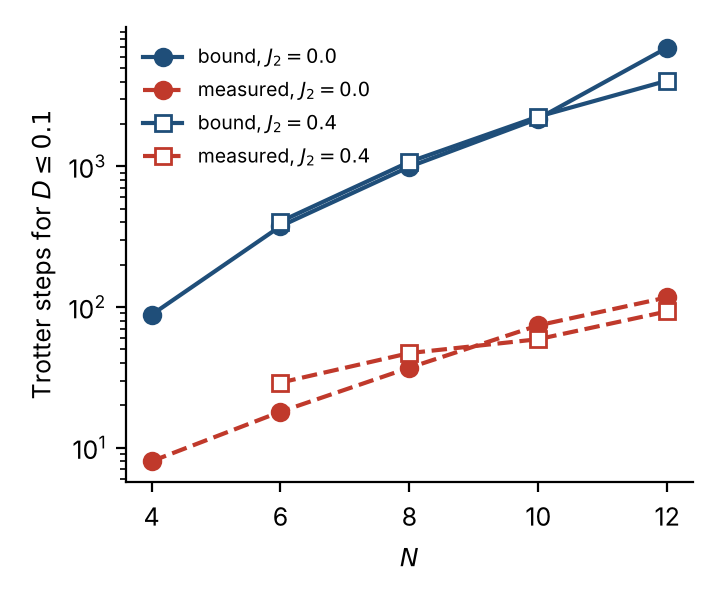
\includegraphics[width=0.55\textwidth,height=\textheight]{figs/fig_steps.png}
\caption{Figure 2. Trotter steps needed for \(D\leq0.1\): prescribed by
the bound (blue) vs.~measured (red), \(\chi=2\).}
\end{figure}

\hypertarget{which-term-is-loose}{%
\subsubsection{5.4 Which term is loose?}\label{which-term-is-loose}}

\begin{longtable}[]{@{}
  >{\raggedright\arraybackslash}p{(\columnwidth - 20\tabcolsep) * \real{0.0909}}
  >{\raggedright\arraybackslash}p{(\columnwidth - 20\tabcolsep) * \real{0.0909}}
  >{\raggedright\arraybackslash}p{(\columnwidth - 20\tabcolsep) * \real{0.0909}}
  >{\raggedright\arraybackslash}p{(\columnwidth - 20\tabcolsep) * \real{0.0909}}
  >{\raggedright\arraybackslash}p{(\columnwidth - 20\tabcolsep) * \real{0.0909}}
  >{\raggedright\arraybackslash}p{(\columnwidth - 20\tabcolsep) * \real{0.0909}}
  >{\raggedright\arraybackslash}p{(\columnwidth - 20\tabcolsep) * \real{0.0909}}
  >{\raggedright\arraybackslash}p{(\columnwidth - 20\tabcolsep) * \real{0.0909}}
  >{\raggedright\arraybackslash}p{(\columnwidth - 20\tabcolsep) * \real{0.0909}}
  >{\raggedright\arraybackslash}p{(\columnwidth - 20\tabcolsep) * \real{0.0909}}
  >{\raggedright\arraybackslash}p{(\columnwidth - 20\tabcolsep) * \real{0.0909}}@{}}
\toprule\noalign{}
\begin{minipage}[b]{\linewidth}\raggedright
\(N\)
\end{minipage} & \begin{minipage}[b]{\linewidth}\raggedright
\(J_2\)
\end{minipage} & \begin{minipage}[b]{\linewidth}\raggedright
\(\bar D_{\mathrm{leak}}\)
\end{minipage} & \begin{minipage}[b]{\linewidth}\raggedright
\(D_{\mathrm{leak}}\)
\end{minipage} & \begin{minipage}[b]{\linewidth}\raggedright
ratio
\end{minipage} & \begin{minipage}[b]{\linewidth}\raggedright
\(\bar D_{\mathrm{Trot}}\)
\end{minipage} & \begin{minipage}[b]{\linewidth}\raggedright
\(D_{\mathrm{Trot}}\)
\end{minipage} & \begin{minipage}[b]{\linewidth}\raggedright
ratio
\end{minipage} & \begin{minipage}[b]{\linewidth}\raggedright
\(D\le D_{\mathrm{leak}}+D_{\mathrm{Trot}}\)
\end{minipage} & \begin{minipage}[b]{\linewidth}\raggedright
\(P_{\mathrm{succ}}\)
\end{minipage} & \begin{minipage}[b]{\linewidth}\raggedright
\(\gamma F(0)^2\)
\end{minipage} \\
\midrule\noalign{}
\endhead
\bottomrule\noalign{}
\endlastfoot
4 & 0.0 & 0.0490 & 0.0194 & 2.52 & 0.0508 & 0.00173 & 29 & yes & 0.627 &
0.629 \\
6 & 0.0 & 0.0490 & 0.0368 & 1.33 & 0.0508 & 0.00259 & 20 & yes & 0.445 &
0.446 \\
6 & 0.4 & 0.0490 & 0.0227 & 2.16 & 0.0506 & 0.00528 & 10 & yes & 0.942 &
0.943 \\
8 & 0.0 & 0.0490 & 0.0320 & 1.53 & 0.0505 & 0.00314 & 16 & yes & 0.356 &
0.357 \\
8 & 0.4 & 0.0490 & 0.0232 & 2.11 & 0.0508 & 0.00273 & 19 & yes & 0.777 &
0.778 \\
10 & 0.0 & 0.0491 & 0.0325 & 1.51 & 0.0502 & 0.00255 & 20 & yes & 0.274
& 0.274 \\
10 & 0.4 & 0.0490 & 0.0200 & 2.45 & 0.0508 & 0.00177 & 29 & yes & 0.650
& 0.650 \\
12 & 0.0 & 0.0494 & 0.0228 & 2.16 & 0.0499 & 0.00128 & 39 & yes & 0.605
& 0.606 \\
12 & 0.4 & 0.0491 & 0.0214 & 2.29 & 0.0508 & 0.00162 & 31 & yes & 0.564
& 0.564 \\
\end{longtable}

\emph{Table 2.} \(\varepsilon=10^{-2}\), at \(n_{\mathrm{bound}}\). Bars
denote the bound; unbarred the measured distance. Last two columns:
measured success probability of the Trotterised filter and the
guaranteed lower bound.

\begin{itemize}
\tightlist
\item
  \textbf{Leakage} is nearly tight: bound/measured \$=\$1.3--2.5. The
  only slack is that every excited component is charged the worst-case
  filter value \(\eta F(0)\).
\item
  \textbf{Trotter} is conservative: 10--39\(\times\). The constant
  \(\alpha\) is a worst case over all states. The companion analysis in
  \texttt{evaluation/} found that the ground state sees a first-order
  Trotter coefficient 28--41\(\times\) smaller than \(\alpha\) at
  \(J_2=0\); we did not re-measure that here.
\item
  \textbf{Total.} The measured \(D\) at \(n_{\mathrm{bound}}\) is
  dominated by leakage (\(D_{\mathrm{leak}}\approx0.02\)--\(0.04\)
  vs.~\(D_{\mathrm{Trot}}\lesssim0.005\)), which is why the bound is
  within a factor 3--5 although the Trotter term alone is loose by
  \(10\)--\(39\times\).
\item
  \textbf{Success probability.} \(P_{\mathrm{succ}}\) agrees with
  \(\gamma F(0)^2\) to 0.6\% (relative), so \(1/(\gamma F(0)^2)\) is an
  accurate estimate of the repetition cost.
\end{itemize}

\begin{figure}
\centering
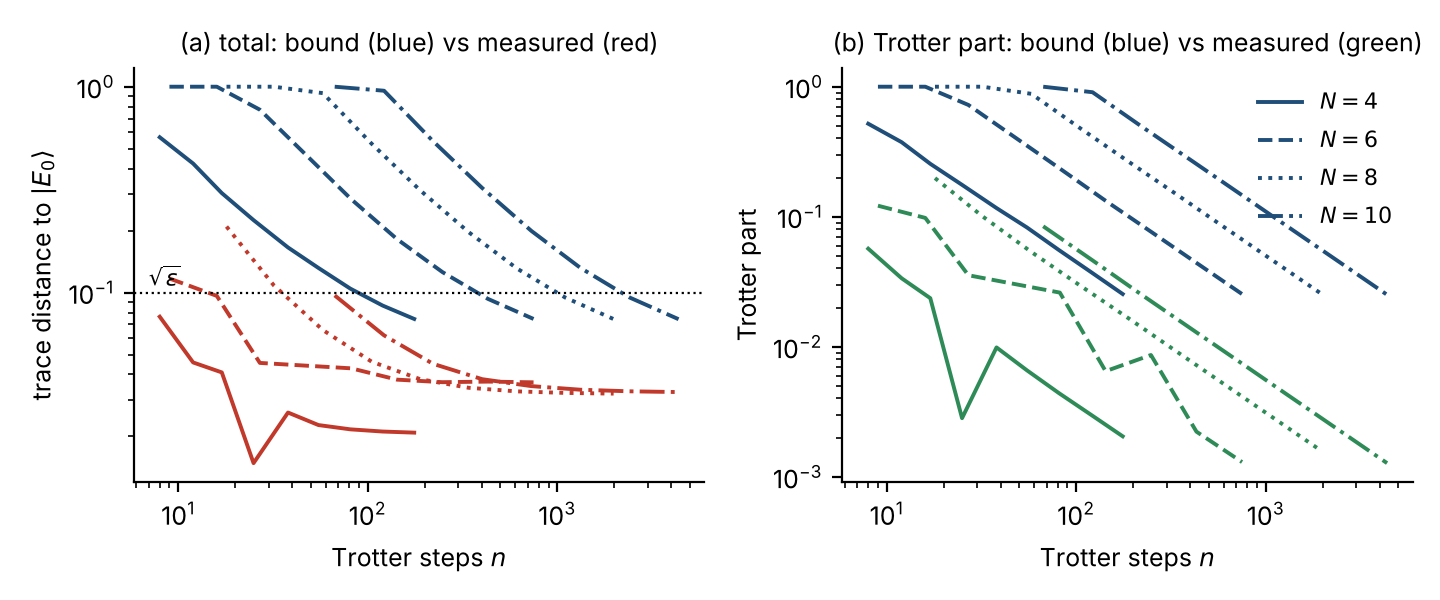
\includegraphics[width=1\textwidth,height=\textheight]{figs/fig_sweep.png}
\caption{Figure 3. Sweep over \(n\) at fixed design,
\(\varepsilon=10^{-2}\), \(J_2=0\), \(N=4,6,8,10\) (solid, dashed,
dotted, dash-dotted). (a) total bound and measured distance; (b) Trotter
part only.}
\end{figure}

\hypertarget{dependence-on-n}{%
\subsubsection{\texorpdfstring{5.5 Dependence on
\(n\)}{5.5 Dependence on n}}\label{dependence-on-n}}

Figure 3 shows the sweep. Both the Trotter bound and the measured
Trotter distance fall as \(1/n\) (fitted log--log slopes \(-0.98\) to
\(-1.01\) for the bound and \(-0.99\) to \(-1.09\) for the measurement,
over the sweep points where the bound is non-trivial, in all 9 sweeps),
so the bound has the right \emph{scaling} in \(n\) and is off by a
roughly constant factor. The measured total distance saturates at the
leakage floor \(D_{\mathrm{leak}}\), as it must: more Trotter steps
cannot reduce leakage. The non-monotone dips at small \(n\) are the
pre-asymptotic regime (\(n\) comparable to the number of pulses).

\hypertarget{observables-and-a-non-oracle-estimate}{%
\subsubsection{5.6 Observables and a non-oracle
estimate}\label{observables-and-a-non-oracle-estimate}}

\begin{longtable}[]{@{}
  >{\raggedright\arraybackslash}p{(\columnwidth - 16\tabcolsep) * \real{0.1111}}
  >{\raggedright\arraybackslash}p{(\columnwidth - 16\tabcolsep) * \real{0.1111}}
  >{\raggedright\arraybackslash}p{(\columnwidth - 16\tabcolsep) * \real{0.1111}}
  >{\raggedright\arraybackslash}p{(\columnwidth - 16\tabcolsep) * \real{0.1111}}
  >{\raggedright\arraybackslash}p{(\columnwidth - 16\tabcolsep) * \real{0.1111}}
  >{\raggedright\arraybackslash}p{(\columnwidth - 16\tabcolsep) * \real{0.1111}}
  >{\raggedright\arraybackslash}p{(\columnwidth - 16\tabcolsep) * \real{0.1111}}
  >{\raggedright\arraybackslash}p{(\columnwidth - 16\tabcolsep) * \real{0.1111}}
  >{\raggedright\arraybackslash}p{(\columnwidth - 16\tabcolsep) * \real{0.1111}}@{}}
\toprule\noalign{}
\begin{minipage}[b]{\linewidth}\raggedright
\(N\)
\end{minipage} & \begin{minipage}[b]{\linewidth}\raggedright
\(J_2\)
\end{minipage} & \begin{minipage}[b]{\linewidth}\raggedright
\(n\)
\end{minipage} & \begin{minipage}[b]{\linewidth}\raggedright
\(\bar D\)
\end{minipage} & \begin{minipage}[b]{\linewidth}\raggedright
\(D\)
\end{minipage} & \begin{minipage}[b]{\linewidth}\raggedright
\(W\bar D^2\)
\end{minipage} & \begin{minipage}[b]{\linewidth}\raggedright
\(\langle H\rangle-E_0\)
\end{minipage} & \begin{minipage}[b]{\linewidth}\raggedright
Richardson \(\hat D_{\mathrm{Trot}}\)
\end{minipage} & \begin{minipage}[b]{\linewidth}\raggedright
\(D_{\mathrm{Trot}}\)
\end{minipage} \\
\midrule\noalign{}
\endhead
\bottomrule\noalign{}
\endlastfoot
4 & 0.0 & 88 & 0.0998 & 0.0202 & 0.0236 & 0.00075 & 0.00177 & 0.00173 \\
6 & 0.0 & 375 & 0.0999 & 0.0365 & 0.0373 & 0.00232 & 0.00259 &
0.00259 \\
6 & 0.4 & 405 & 0.0996 & 0.0256 & 0.0388 & 0.00088 & 0.0053 & 0.00528 \\
8 & 0.0 & 992 & 0.0996 & 0.0326 & 0.0508 & 0.00164 & 0.00314 &
0.00314 \\
8 & 0.4 & 1075 & 0.0999 & 0.0243 & 0.0536 & 0.00074 & 0.00273 &
0.00273 \\
10 & 0.0 & 2183 & 0.0993 & 0.0332 & 0.0642 & 0.00154 & 0.00255 &
0.00255 \\
10 & 0.4 & 2256 & 0.0998 & 0.0208 & 0.0681 & 0.00038 & 0.00177 &
0.00177 \\
12 & 0.0 & 6967 & 0.0993 & 0.0227 & 0.0778 & 0.00073 & -- & 0.00128 \\
12 & 0.4 & 4060 & 0.0998 & 0.0221 & 0.0827 & 0.00038 & 0.00162 &
0.00162 \\
\end{longtable}

\emph{Table 3.} \(\varepsilon=10^{-2}\) at \(n_{\mathrm{bound}}\).
Energy bound (Corollary 2) vs.~measured energy error; and a
Richardson-type Trotter estimate
\(\hat D_{\mathrm{Trot}}=2\,D(\tilde\varphi_n,\tilde\varphi_{2n})\),
which compares the same filter at \(n\) and \(2n\) steps and does not
use \(|g\rangle\).

\begin{itemize}
\tightlist
\item
  \textbf{Energy.} Corollary 2 holds but is conservative by
  16--217\(\times\), because the bound charges every unit of excited
  weight the full bandwidth \(W\).
\item
  \textbf{Richardson estimate.} Across the 60 sweep points with
  \(n\ge n_{\mathrm{emp}}\) the ratio
  \(\hat D_{\mathrm{Trot}}/D_{\mathrm{Trot}}\) lies in {[}0.84, 1.07{]}
  (median 1.00). It is an \emph{estimate}, not a bound: it assumes the
  error vector scales as \(1/n\). It is the natural practical complement
  to Theorem 1, giving a rigorous leakage term plus an empirical Trotter
  term.
\end{itemize}

\textbf{Effect of the trial state.} At \(N=8\), \(J_2=0\),
\(\varepsilon=10^{-2}\):

\begin{longtable}[]{@{}
  >{\raggedright\arraybackslash}p{(\columnwidth - 16\tabcolsep) * \real{0.1111}}
  >{\raggedright\arraybackslash}p{(\columnwidth - 16\tabcolsep) * \real{0.1111}}
  >{\raggedright\arraybackslash}p{(\columnwidth - 16\tabcolsep) * \real{0.1111}}
  >{\raggedright\arraybackslash}p{(\columnwidth - 16\tabcolsep) * \real{0.1111}}
  >{\raggedright\arraybackslash}p{(\columnwidth - 16\tabcolsep) * \real{0.1111}}
  >{\raggedright\arraybackslash}p{(\columnwidth - 16\tabcolsep) * \real{0.1111}}
  >{\raggedright\arraybackslash}p{(\columnwidth - 16\tabcolsep) * \real{0.1111}}
  >{\raggedright\arraybackslash}p{(\columnwidth - 16\tabcolsep) * \real{0.1111}}
  >{\raggedright\arraybackslash}p{(\columnwidth - 16\tabcolsep) * \real{0.1111}}@{}}
\toprule\noalign{}
\begin{minipage}[b]{\linewidth}\raggedright
\(\chi\)
\end{minipage} & \begin{minipage}[b]{\linewidth}\raggedright
\(\gamma\)
\end{minipage} & \begin{minipage}[b]{\linewidth}\raggedright
\(\sqrt{1-\gamma}\) (trial)
\end{minipage} & \begin{minipage}[b]{\linewidth}\raggedright
\(T\)
\end{minipage} & \begin{minipage}[b]{\linewidth}\raggedright
\(\eta\)
\end{minipage} & \begin{minipage}[b]{\linewidth}\raggedright
\(n_{\mathrm{bound}}\)
\end{minipage} & \begin{minipage}[b]{\linewidth}\raggedright
\(n_{\mathrm{emp}}\)
\end{minipage} & \begin{minipage}[b]{\linewidth}\raggedright
bound \(\bar D\)
\end{minipage} & \begin{minipage}[b]{\linewidth}\raggedright
measured \(D\)
\end{minipage} \\
\midrule\noalign{}
\endhead
\bottomrule\noalign{}
\endlastfoot
1 & 0.1336 & 0.931 & 41.0 & 0.019 & 8519 & 93 & 0.0993 & 0.0330 \\
2 & 0.8371 & 0.404 & 24.6 & 0.111 & 992 & 37 & 0.0996 & 0.0326 \\
3 & 0.9110 & 0.298 & 24.6 & 0.157 & 877 & 37 & 0.0995 & 0.0214 \\
4 & 0.9988 & 0.035 & -- & -- & no filter needed & -- & -- & 0.035 \\
\end{longtable}

\emph{Table 4.} A better trial state needs fewer Trotter steps (larger
\(\gamma\) means a larger \(\eta_*\), so a shorter, cheaper filter), and
for \(\chi=4\) (\(\gamma=0.9988\)) no filter is needed at this target.

\hypertarget{pinsker-numerics}{%
\subsubsection{5.7 Pinsker numerics}\label{pinsker-numerics}}

For \(\chi=2\), \(\varepsilon=10^{-2}\) and
\((N,J_2)\in\{(4,0),(6,0),(8,0),(6,0.4),(8,0.4)\}\), the energy-resolved
quantities of Section 3.5 (computed for the continuous filter designs
and the exact filter) satisfy
\(\mathrm{KL}(q\|p)\le\ln(1/P_{\mathrm{succ}})\) and
\(\mathrm{TV}(p,q)\le\sqrt{\mathrm{KL}/2}\) in every case, as they must.
The implied cap on the success probability,
\(\exp(-2(1-\ell-\gamma)^2)\), is \(0.95\)--\(1.00\), against actual
\(P_{\mathrm{succ}}\) between \(0.36\) and \(0.94\). It is true but too
weak to be informative for these trial states, which already have large
\(\gamma\). We therefore treat Pinsker as an explanatory remark, not as
part of the guarantee.

\hypertarget{discussion-and-limitations}{%
\subsection{6. Discussion and
limitations}\label{discussion-and-limitations}}

\begin{itemize}
\tightlist
\item
  \textbf{Inputs.} The bound is conditional on exact \(\gamma\) and
  \(\Delta\) (and \(E_0\) for the shift). Here they come from exact
  diagonalisation, so everything is restricted to \(N\le12\). At larger
  \(N\) the energies come from DMRG, which gives estimates, not bounds:
  the penalty-method first-excitation energy is an \emph{upper} bound on
  \(E_1\), the wrong side for a gap lower bound, and an overlap with a
  DMRG state is an overlap with an approximation of \(|E_0\rangle\).
  Certifying \(\Delta\) and \(\gamma\) at large \(N\) is the main open
  point for turning this into a large-\(N\) workflow.
\item
  \textbf{Trial state.} The trial states are SVD truncations of the
  exact ground state standing in for DMRG/MPS-circuit states. Circuit
  compilation would reduce \(\gamma\) further; the bound applies
  unchanged given the true \(\gamma\).
\item
  \textbf{First order only.} Lemma 2 is a first-order product-formula
  statement.
\item
  \textbf{Conservatism.} The Trotter term is the loose one (10--39×).
  Using the Richardson estimate in its place gives a practical,
  non-rigorous complement.
\item
  \textbf{Noise.} Not modelled; (D2) adds a noise term as in Section
  3.5.
\item
  \textbf{Cost.} We report steps, not CX or T counts, and make no claim
  of advantage over direct MPS-circuit preparation (see the companion
  study).
\item
  \textbf{Scale.} \(N\le12\), two couplings, dense simulation.
\end{itemize}

\hypertarget{reproducibility}{%
\subsection{7. Reproducibility}\label{reproducibility}}

Everything is in \texttt{simple\_paper/}: \texttt{workflow.py}
(Hamiltonian, trial state, pulses, bound), \texttt{run\_experiments.py}
(cases, writes \texttt{results/case\_*.json}),
\texttt{pinsker\_check.py}, \texttt{make\_report.py} (tables, figures),
\texttt{build\_paper.py} (this document). The filter design and
certification are \texttt{j1j2\_filter/floor.py}. Requirements: numpy,
scipy, matplotlib; no qiskit or quimb. The full grid takes a few minutes
on one CPU core (the \(N=12\) cases dominate). Seeds are fixed (the
\(N=12\) ground state uses a fixed Lanczos start vector, since
\(\chi=2\) truncation cuts through degenerate Schmidt values and
\(\gamma\) otherwise varies in the third digit between runs).

\hypertarget{references}{%
\subsection{References}\label{references}}

\begin{enumerate}
\def\labelenumi{\arabic{enumi}.}
\tightlist
\item
  I. Stetcu, A. Baroni, J. Carlson, ``Projection algorithm for state
  preparation on quantum computers,'' \emph{Phys. Rev.~C} \textbf{105},
  064308 (2022).
\item
  K. Choi, D. Lee, J. Bonitati, Z. Qian, J. Watkins, ``Rodeo algorithm
  for quantum computing,'' \emph{Phys. Rev.~Lett.} \textbf{127}, 040505
  (2021).
\item
  A. M. Childs, Y. Su, M. C. Tran, N. Wiebe, S. Zhu, ``Theory of Trotter
  error with commutator scaling,'' \emph{Phys. Rev.~X} \textbf{11},
  011020 (2021).
\item
  M. A. Nielsen, I. L. Chuang, \emph{Quantum Computation and Quantum
  Information} (Cambridge University Press, 2000), Ch. 9 (trace
  distance, fidelity).
\item
  C. A. Fuchs, J. van de Graaf, ``Cryptographic distinguishability
  measures for quantum-mechanical states,'' \emph{IEEE Trans. Inf.
  Theory} \textbf{45}, 1216 (1999).
\item
  T. M. Cover, J. A. Thomas, \emph{Elements of Information Theory}
  (Wiley, 2006), Lemma 11.6.1 (Pinsker's inequality).
\item
  S. R. White, ``Density matrix formulation for quantum renormalization
  groups,'' \emph{Phys. Rev.~Lett.} \textbf{69}, 2863 (1992); U.
  Schollwöck, ``The density-matrix renormalization group in the age of
  matrix product states,'' \emph{Ann. Phys.} \textbf{326}, 96 (2011).
\end{enumerate}

\hypertarget{appendix-a.-first-order-trotter-bound}{%
\subsection{Appendix A. First-order Trotter
bound}\label{appendix-a.-first-order-trotter-bound}}

\textbf{Two terms.} For Hermitian \(A,B\), \(U(s)=e^{-is(A+B)}\) and
\(V(s)=e^{-isA}e^{-isB}\):
\(\frac{d}{ds}[U(\delta-s)V(s)]=iU(\delta-s)\big(B-e^{-isA}Be^{isA}\big)V(s)\),
so integrating from \(0\) to \(\delta\),
\[U(\delta)-V(\delta)=-i\int_0^\delta U(\delta-s)\big(B-e^{-isA}Be^{isA}\big)V(s)\,ds .\]
Since \(\frac{d}{ds}e^{-isA}Be^{isA}=-ie^{-isA}[A,B]e^{isA}\), we have
\(\|B-e^{-isA}Be^{isA}\|\le s\|[A,B]\|\), and \(U,V\) are unitary, so
\(\|U(\delta)-V(\delta)\|\le\tfrac{\delta^2}{2}\|[A,B]\|\).

\textbf{Many terms.} For \(H=H_1+\dots+H_\Gamma\) and the product
\(S=e^{-i\delta H_1}\cdots e^{-i\delta H_\Gamma}\), apply the two-term
bound with \(A=H_1\), \(B=R_1:=\sum_{g>1}H_g\) and recurse on
\(e^{-i\delta R_1}\) versus the product of the rest (unitary invariance
of the norm absorbs the leading factor):
\[\big\|e^{-i\delta H}-S\big\|\le\frac{\delta^2}{2}\sum_{g}\Big\|\Big[H_g,\sum_{g'>g}H_{g'}\Big]\Big\|=\frac{\delta^2}{2}\alpha .\]
With \(\delta=t/k\) and \(k\) steps, \(\|X^k-Y^k\|\le k\|X-Y\|\) gives
\(\alpha t^2/(2k)\). The opposite product order gives the reversed sum;
the code takes the larger of the two. This is the first-order case of
Childs et al.~{[}3{]}.

\textbf{Ancilla.} For \(H_s\otimes Z\) the terms are \(H_gZ\), and
\([H_gZ,H_{g'}Z]=[H_g,H_{g'}]\otimes Z^2=[H_g,H_{g'}]\otimes\mathbb 1\),
so \(\alpha\) is unchanged. The constant shift \(-E_0/W\) commutes with
everything and is applied exactly.

\end{document}
